\documentclass[twocolumn, 12pt]{article}
\usepackage[letterpaper, margin = 0.5in]{geometry}
\usepackage{lmodern}
\usepackage[english,activeacute]{babel}
\usepackage{mathtools}
\usepackage{graphicx}
\usepackage{subcaption}
\usepackage{amsmath}
\usepackage{amsfonts}
\usepackage{amssymb}
\usepackage{enumitem,kantlipsum}

\title{Guided Capstone Project Report}
\author{Big Mountain Resort}

\begin{document}

\maketitle

\section{Ticket Price Calculation}

\noindent
The model that was created took into account the following features which are listed from the most important to the least:

\begin{itemize}
	\item Vertical Drop.
	\item Snow making acres.
	\item Total number of chairs.
	\item Number of \textit{Fast Quads}.
	\item Number of runs.
	\item Number of miles of the longest run.
	\item Skiable terrain.
\end{itemize}

We can see that it is the vertical drop as well as the snow making acres the two features that have the strongest influence upon the predictions of the model for the ticket price.\linebreak


Using the model with the provided data, the predicted price is $ \$98.07 $ with an absolute mean error of $ \$ 10.46 $. This prediction infers that it is possible that our resort may be undercharging since the present ticket price is $ \$81.00 $.
	
\section{Locating Big Mountain Resort in Market Context}

\begin{figure}[h!]
	\centering
	\begin{subfigure}[b]{0.48\linewidth}
		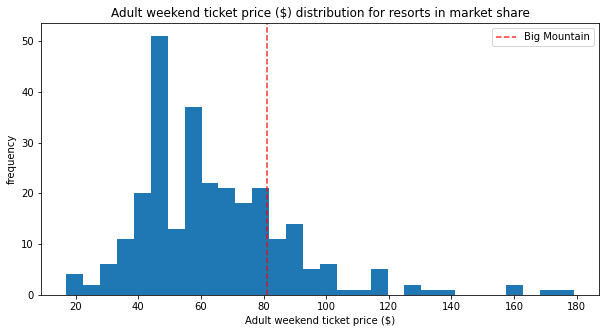
\includegraphics[width=\linewidth]{weekendprice.png}
		\caption{All resorts}
	\end{subfigure}
	\begin{subfigure}[b]{0.48\linewidth}
		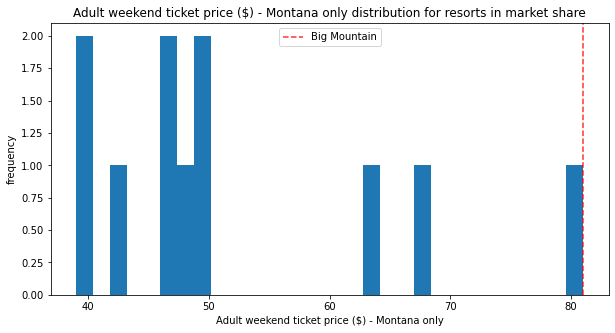
\includegraphics[width=\linewidth]{weekendpricemontana.png}
		\caption{Resorts in Montana}
	\end{subfigure}
	\caption{Weekend prices in the Market}
	\label{weekendprices}
\end{figure}

\noindent
Figures (\ref{weekendprices}) to (\ref{skiableterrain}) let us know where Big Mountain sits in the distribution of each of the features listed above. This helps us understand and justify a ticket price increase. Figure (\ref{weekendprices}) shows that Big Mountain's ticket price is above the mean market price and is above the price of all the resorts in Montana. \linebreak

\begin{figure}[!htb]
	\begin{minipage}{0.24\textwidth}
		\centering
		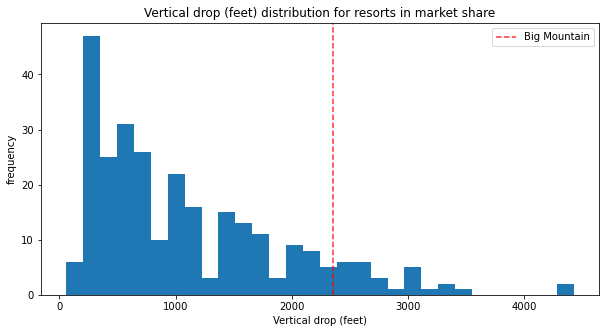
\includegraphics[width=\linewidth]{verticaldrop.png}
		\caption{Vertical drop}\label{verticaldrop}
	\end{minipage}\hfill
	\begin {minipage}{0.24\textwidth}
	\centering
	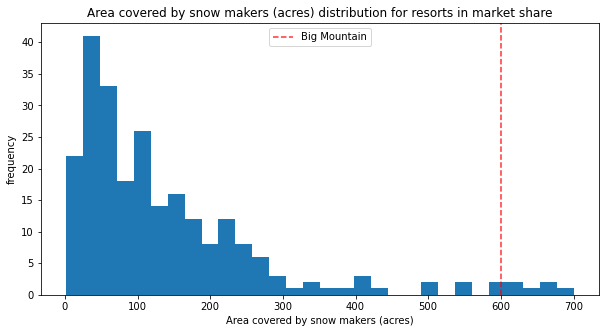
\includegraphics[width=\linewidth]{snowcoveredarea.png}
	\caption{Snow covered area}\label{snowcoveredarea}
\end{minipage}
\end{figure}

Figures (\ref{verticaldrop}) to (\ref{skiableterrain}) show us that Big Mountain is among the most resourceful resorts in the market. In particular, it has one of the highest vertical drops in the market and had also has one of the greatest areas covered by snow making machines. 

\begin{figure}[!htb]
	\begin{minipage}{0.24\textwidth}
		\centering
		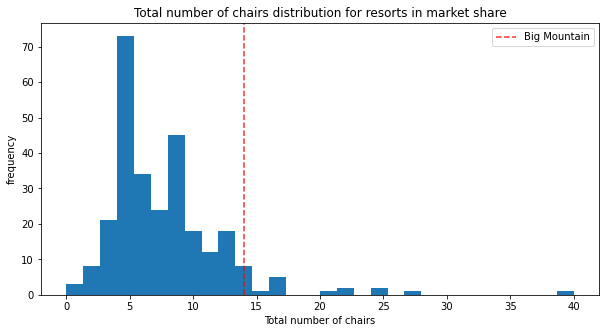
\includegraphics[width=\linewidth]{numberchairs.png}
		\caption{Vertical drop}\label{numberchairs}
	\end{minipage}\hfill
	\begin {minipage}{0.24\textwidth}
	\centering
	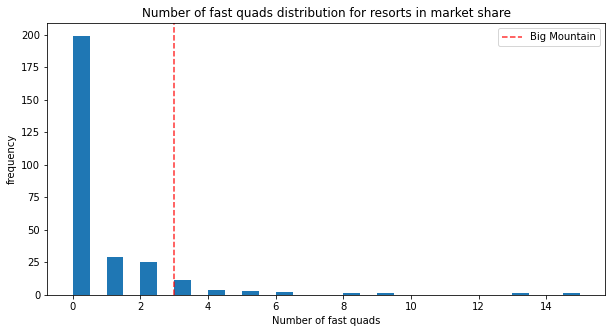
\includegraphics[width=\linewidth]{fastquads.png}
	\caption{Number of Fast Quads}\label{fastquads}
\end{minipage}
\end{figure}


\begin{figure}[!htb]
	\begin{minipage}{0.24\textwidth}
		\centering
		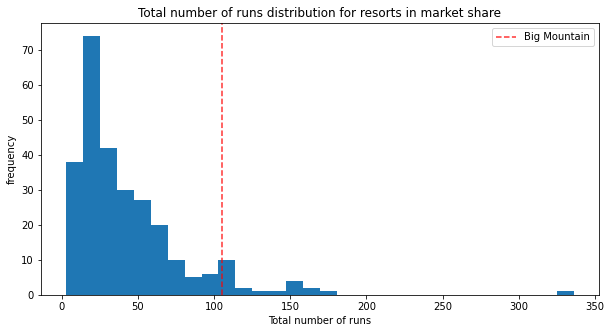
\includegraphics[width=\linewidth]{totalnumberruns.png}
		\caption{Number of runs}\label{numberruns}
	\end{minipage}\hfill
	\begin {minipage}{0.24\textwidth}
	\centering
	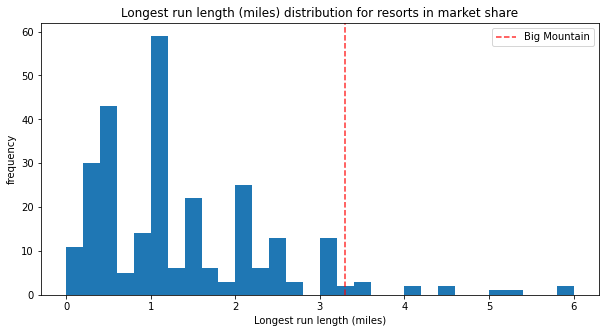
\includegraphics[width=\linewidth]{longestrun.png}
	\caption{Length of longest run}\label{runlength}
	\end{minipage}
\end{figure}

This means that Big Mountain is one of the few that can guarantee snow any time of the year at the same time that offers tourists an attractive and competitive vertical drop. This two features showed to be heavily correlated with the ticket price.  \linebreak \linebreak \linebreak

\begin{figure}[!htb]
	\begin{minipage}{0.24\textwidth}
		\centering
		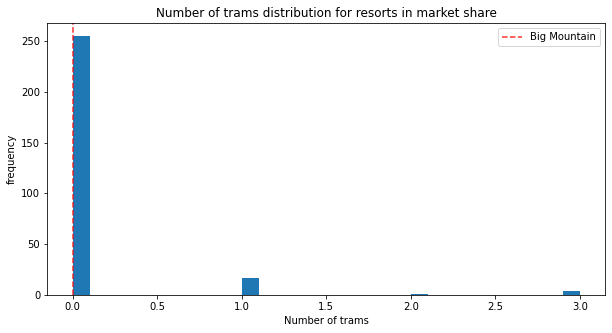
\includegraphics[width=\linewidth]{numbertrams.png}
		\caption{Number of trams}\label{numbertrams}
	\end{minipage}\hfill
	\begin {minipage}{0.24\textwidth}
	\centering
	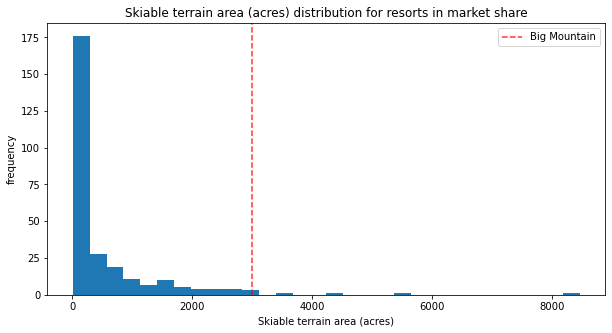
\includegraphics[width=\linewidth]{skiableterrainarea.png}
	\caption{Skiable Terrain}\label{skiableterrain}
\end{minipage}
\end{figure}

Considering that Big Mountain is ranking high with respect to the rest of the features, it is possible to consider an increase in the ticket price that could take into account the resort's equipment and characteristics.

\section{Suggeted Alternatives}

\noindent
Big Mountain resort has been reviewing potential scenarios for either cutting costs or increasing revenue. In order to make our calculations, we considered number of visitors of $350,00$ over the season. The average amount of time that  vistors stay is five days. Taking the previous data into account, the following options were considered:

\begin{itemize}
	\item \textbf{Permanently closing down up to ten of the least used runs:} This strategy leads to reducing support for ticket price as we can see in Figure (\ref{scenario1}).
	
	\begin{figure}[h!]
		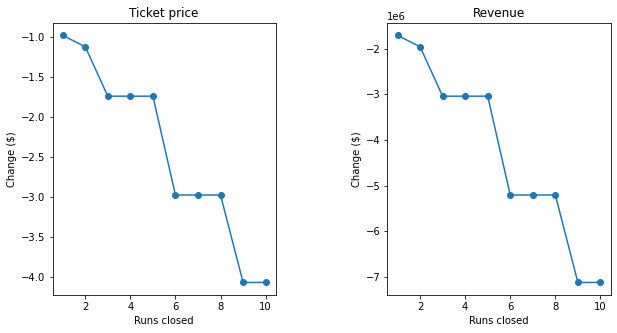
\includegraphics[width=\linewidth]{scenario1.png}
		\caption{Increase in ticket price with increasing number of closed runs.} 
		\label{scenario1}
	\end{figure}
	
	\item \textbf{Increase the vertical drop by adding a run to a point 150 lower down, requiring the installation of an additional chair lift without additional snow coverage:} For this scenario, the model predicts an increase in the support for the ticket price of $ \$1.55 $. Over the season, this would imply an expected increase in total income of $ \$2,708,333$.
	
	\item \textbf{Increase the vertical drop in the same way that is suggested on the previous scenario but by adding 2 acres of snow cover:} This scenario leads to exactly the same results as the previous one.
	
	\item \textbf{Increase the lowest run by 0.2 mile to boast 3.5 length, requiring addtional snow-making coverage of 4 acres:} The model predicts that this improvement will have no effect on ticket price and no increase at all would be registered. 
\end{itemize}

\end{document}